\chapter{Outlook}
\section{Concept and work planning for the continuation}

As a result of the previous project work (see section \ref{sec:geomint}), a broad experimental and numerical platform for the investigation of discontinuities due to swelling and shrinking processes (WP1), pressure-driven percolation (WP2) and stress redistribution (WP3) has been developed. The most important barrier and reservoir rocks (clay, salt, crystalline) will be recorded. A comprehensive validation of the platforms (\glqq{}Proof-of-Concept\grqq) was carried out by model experiments (MEX) for the damage and fracture processes driven by different processes (see chapter \ref{cha:mex}).
In the planned continuation of the project the basic idea -- the investigation of the three relevant process types for the formation of pathways in different rock types -- shall be preserved. The proven project structure (WP1-3) is also to be retained (Fig. \ref{fig:pro02}).
%
After a very strongly methodically oriented first phase, the continuation project is intended to demonstrate practical applicability under real conditions (URLs). Furthermore, knowledge gaps in the experimental as well as numerical field shall be closed.

The \textbf{focus in GeomInt2} is done as follows:
\begin{list}{--}{\leftmargin=1em \itemindent=0em \itemsep=-0.5em}
\item experiments: The focus is on the evaluation of the latest in-situ experiments in the rock\-laboratories Mt. Terri (Opalinus clay), Springen (salt) and Reiche Zeche (crystalline). Selected laboratory experiments are planned in order to specifically close still existing knowledge gaps (e.g. mechanical anisotropy of clay rocks).
\item modelling: Numerical methods are to be further developed and applied for in-situ use in a focused manner. For the scaling from micro- to macroscale models, different model approaches are to be specifically linked together (e.g. integration of the LEM in the FE method).
\item digitization: New developments in computer science, such as high-performance computing and visual data analysis, will be incorporated into the continuation of the project. This is necessary on the one hand to achieve the necessary scaling of the models (from micro to macro scale) and on the other hand to allow the representation of the model results in the real context of the underground laboratories.
\item Internationalization: In addition, international cooperation with the Mt. Terri project and DECOVALEX 2023 will be intensified, also to increase the visibility of the Geo:N project.
\end{list}

\section{AP1: Pathways through swelling and shrinking processes (BGR, TUBAF, UFZ, CAU)}
\label{sec:wp1-plan}

\begin{wrapfigure}{l}{0.5\textwidth}
\vspace{-5mm}
\centering
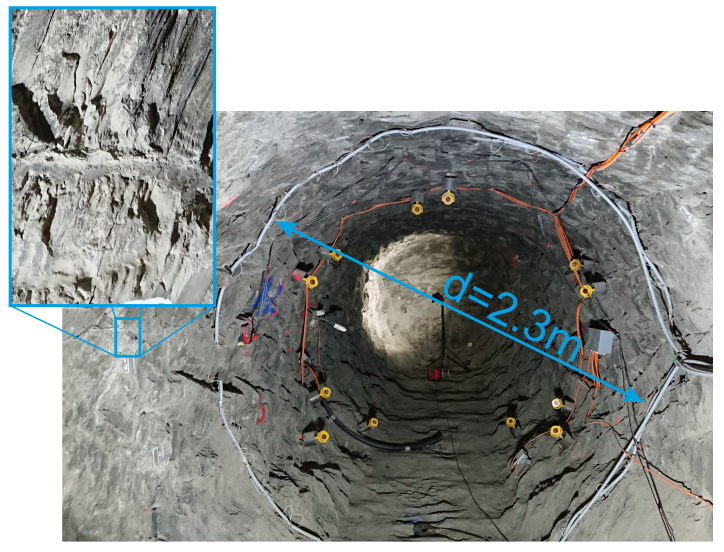
\includegraphics[width=0.49\textwidth]{figures/CDA_open_niche}
\caption{URL Mt. Terri: CD-A experiment: desaturation cracks at the ventilated open niche (Photo: BGR)}
\label{fig:cd-a}
\end{wrapfigure}
The focus of the work in the continuation is the Mt. Terri CD-A experiment. In autumn 2019, two 11\,m long niches were excavated and extensively instrumented. While one niche is ventilated and thus exposed to seasonal fluctuations in humidity, the second niche is kept closed by a bulkhead. First geophysical measurements as well as observations of drying cracks on the walls already indicate the influence of desaturation in the ventilated niche, while the closed niche, where a constantly high humidity has been established, does not show any such cracks. Based on the experimental analyses, the anisotropic swelling and shrinking behaviour under these boundary conditions is analysed and characterised in the laboratory. The analysis is the basis for further modelling on larger scales. 
The numerical methods \cite{Yoshioka2019,Parisio2019102} developed in GeomInt are to be used and, if necessary, further refined in order to model and analyse the observed differences between the two niches. In a first step, the two-dimensional HM calculations of the CD/LP experiment (in \cite{Kolditz2020b}) performed within GeomInt will be extended by the newly developed non-linear transversal-isotropic approaches in mechanics and in the swelling and shrinking model. Furthermore, the possibility of modelling shrinkage cracks in the HM context is investigated on the mechanical side by the phase field method and plastic models and on the hydraulic side with multicontinua models. In a second step, this approach will be applied to the CD-A experiment and quantitatively analyzed by comparison with measured data, so that a basic validation of the model approach on field scale is possible. 

\section{AP2: Displacements due to pressure-driven percolation}

\subsection{Pressure-driven percolation in clay rock under in-situ conditions}

\begin{wrapfigure}{l}{0.5\textwidth}
\vspace{-5mm}
\centering
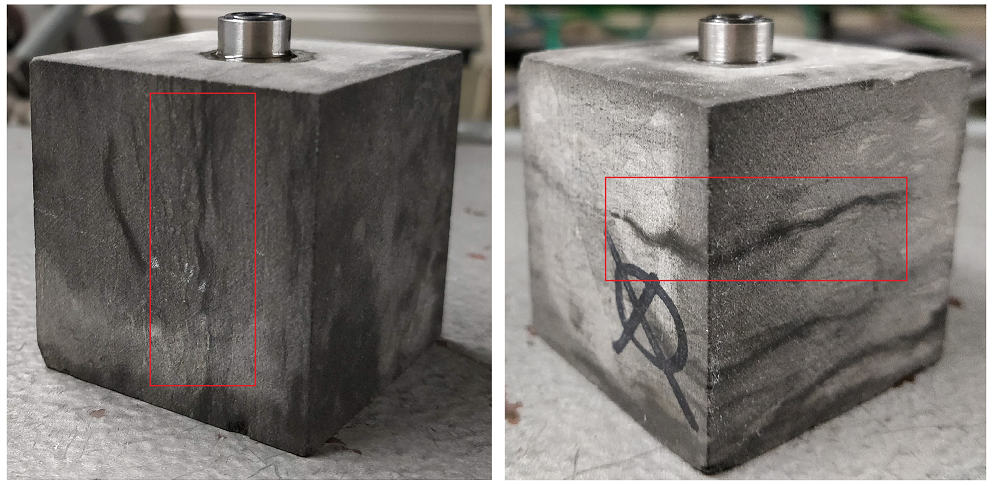
\includegraphics[width=0.49\textwidth]{figures/GeomInt_AP2_CAU}
\caption{Pathways through pressure-driven percolation, clay rock (Photo: CAU Kiel)}
\label{fig:cd-a}
\end{wrapfigure}
In the GeomInt continuation, the laboratory-experimental focus is on the investigation of anisotropy effects. This material state determines all physical properties, especially for claystone. For the characterization of the anisotropic material behavior, in particular fracture behavior and pathability under temperature, saturation and pressure changes are to be analyzed. Selected investigations, e.g. fracture toughness analyses, fluid-driven percolation tests or high-pressure cube pressure tests are to be carried out with special consideration of the material anisotropy. Any additional material samples that may be required could be provided by ongoing drilling activities in the new galleries in the Mt. Terri rock laboratory. The aim is to determine the anisotropic fracture and strength parameters, conductivities or fracture paths required for further simulations during fluid percolation under in-situ conditions.

The already developed thermo-hydro-break-mechanical lattice element method (LEM) is used with a vectorized meshing for anisotropic boundary conditions and verified by the above mentioned specific laboratory tests. 
%
For the transition from micro- or mesoscale LEM to macroscale FEM simulations, the \glqq Mesh Fragmentation Technique (MFT)\grqq{} is to be extended in such a way that vectorized Voronoi LEM grids are directly transferred to the finite element meshes according to the MFT. The material properties of the MFT interface elements are then replaced by the physical fracture properties of the lattice beams. Since a pre-definition of the crack path is not necessary with this approach even in large scale FE models, this approach is extremely attractive for future realistic simulations.
%
The planned combination of LEM with FEM and thus a consideration of micro-properties for larger scale simulations corresponds to the concept of the GeomInt continuation regarding scaling from laboratory to in-situ scale and thus the direct use of the GeomInt2 modeling platform for URL experiments.

The LIE method \cite{Vowinckel2020}, which has been further developed in GeomInt, will also be used to simulate pressure-driven crevice reactivation in another Mt. Terri experiment (Fault-Slip FS experiment). The hydromechanical coupling is investigated in the case of an inelastic change in the properties of an existing fissure or crack network in the claystone as a result of fluid injection. Due to the special boundary conditions, modeling is of particular importance for the interpretation of this complex in-situ experiment, since the observed behavior in laboratory experiments can only be simulated in a very simplified way.

\subsection{Pressure-driven percolation in salt rock under in-situ conditions}

\begin{wrapfigure}{l}{0.5\textwidth}
\vspace{-5mm}
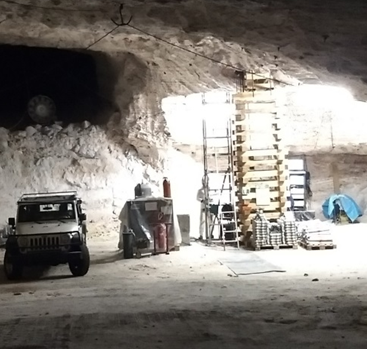
\includegraphics[width=0.49\textwidth]{figures/Versuch-Photo.png}
\caption{Underground laboratory Springen}
\end{wrapfigure}
In the in-situ laboratory of the Springen mine, a large bore hole of 50\,m$^3$ is used to investigate the pressure-driven percolation of both liquids and gases. This was carried out with compressed air, representative of natural gas, and the rupture of the rock was monitored by an array of sensors for acoustic emissions. This large-scale experiment will be evaluated in two ways in the continuation. On the one hand, the influence of the local stress field and the rupture zone on pressure development and propagation direction shall be investigated by means of a discontinuum mechanical method. On the other hand, it shall be determined whether the same process can be reproduced with a continuum mechanical method. The model application is again driven by the idea of scaling from the smaller to the larger in-situ scale.
As an extended continuum mechanical approach, the phase field method is used to simulate the large-scale Springen experiment. 
%
It is planned to compare the two methods (FLAC3D and OpenGeoSys phase field method) with regard to their suitability for scalability to larger systems. This will also involve computational efficiency using HPC methods (parallelisation).

\section{WP3: Displacements due to stress redistribution}

In the continuation of the project, there is the chance to observe on a smaller scale selected phenomena of the hydro-mechanically coupled behaviour of discontinuities, which were integrally investigated in the previous work package, i.e. averaged over the size of the sample on the cm to dm scale. For this purpose, test paths for mechanical and hydraulic scenarios can be built up on the experimental basis already developed with regard to the boundary conditions. 
In particular, the discretization of the shear surfaces with the aid of the 3D scanner represents the link between the measured hydro-mechanically coupled fracture behaviour and local phenomena in the mm range. 
%
Methodologically, a further development towards observational procedures, which allow an appropriate spatial resolution (at least in the mm range) with simultaneous mechanical or coupled loading of the fissure body sample, is being carried out. Specifically, the shear box of the shear apparatus in the Freiberg laboratory is modified in such a way that the arrangement of piezoceramic sensors for recording acoustic emissions (AE) and the fixing of micro-accelerometers directly next to, or above and below the fissure surface is possible. By operating the AE sensors in active mode, i.e. as ultrasonic actuators for pulse generation, damage parallel to the fissure surface and dislocation on the fissure surface can be quantified. The combined use of the AE system and the microseismic network significantly improves the possibilities for locating the damage processes and for generating the hearth surface solution, since shear waves can now also be reliably detected in their 3D spatial position. In contrast to AE sensors, the micro-accelerometers also provide measurement data on the absolute energy of the recorded seismic events, thus enabling quantitative analysis of the crack initiation process in its spatio-temporal evolution.

The gneiss from Freiberg (URL Reiche Zeche) is selected as sample material, with the focus primarily on fissures and fault zones in the otherwise massive gneiss body. Since preliminary tests showed that the foliation of the gneiss is mechanically visible but hydraulically only of limited relevance, crevasses and fault zones were identified as potential pathways in the gneiss.
%
The Freiberg data from the experimental tests are directly used by the Stuttgart team for numerical simulation to characterize the hydro-mechanical coupling of fluid-saturated cracks or fracture networks (using hybrid FE methods). Transient stimulation experiments will be simulated. The combination of e.g. harmonic pump experiments and the numerical simulation tools developed here allows a realistic description of the pressure-dependent effective permeability of the crack networks as well as an estimation of the associated effective crack storage capacity.

This research focus will also strengthen the international networking of GeomInt2 with the DECOVALEX 2023 project. There it is planned to work on complementary objectives to the work package described here - for example, on fissure behavior under thermal or polyaxial boundary conditions. 

Both projects GeomInt2 and STIMTEC2 want to strengthen their cooperation in the continuation. Of great interest for GeomInt2 are the experimental stimulation experiments of the STIMTEC project in the rich coal mine \cite{steeb-2020c} for testing the modeling platform under in-situ conditions. For STIMTEC2 the determination of mechanical and hydraulic properties for the crystalline (characterization of fault zones, fractures and rock matrix) from the GeomInt2 concept is of particular interest. Thus both projects can create significant added value in the cooperation.

%Eine internationale Zusammenarbeit ist auch in der Zukunft weiterhin geplant. Hierzu sollen ebenfalls  Stimulationsexperimente im geklüfteten kristallinen Gestein (Grimsel) vertiefend ausgewertet und untersucht werden, vgl. aktuelle Kooperation \cite{steeb-2020b}.

\section{WP4: Data and model integration using virtualization and high-performance computing}

In the context of the follow-up project, the synthesis activities are to be strengthened. In particular, modern methods of digitization will be further developed and applied. This includes scientific software development, virtualization and high-performance computing - which will be applied specifically to selected GeomInt studies in the sense of demonstrating the GeomInt platform.

\begin{wrapfigure}{l}{0.5\textwidth}
\vspace{-5mm}
\centering
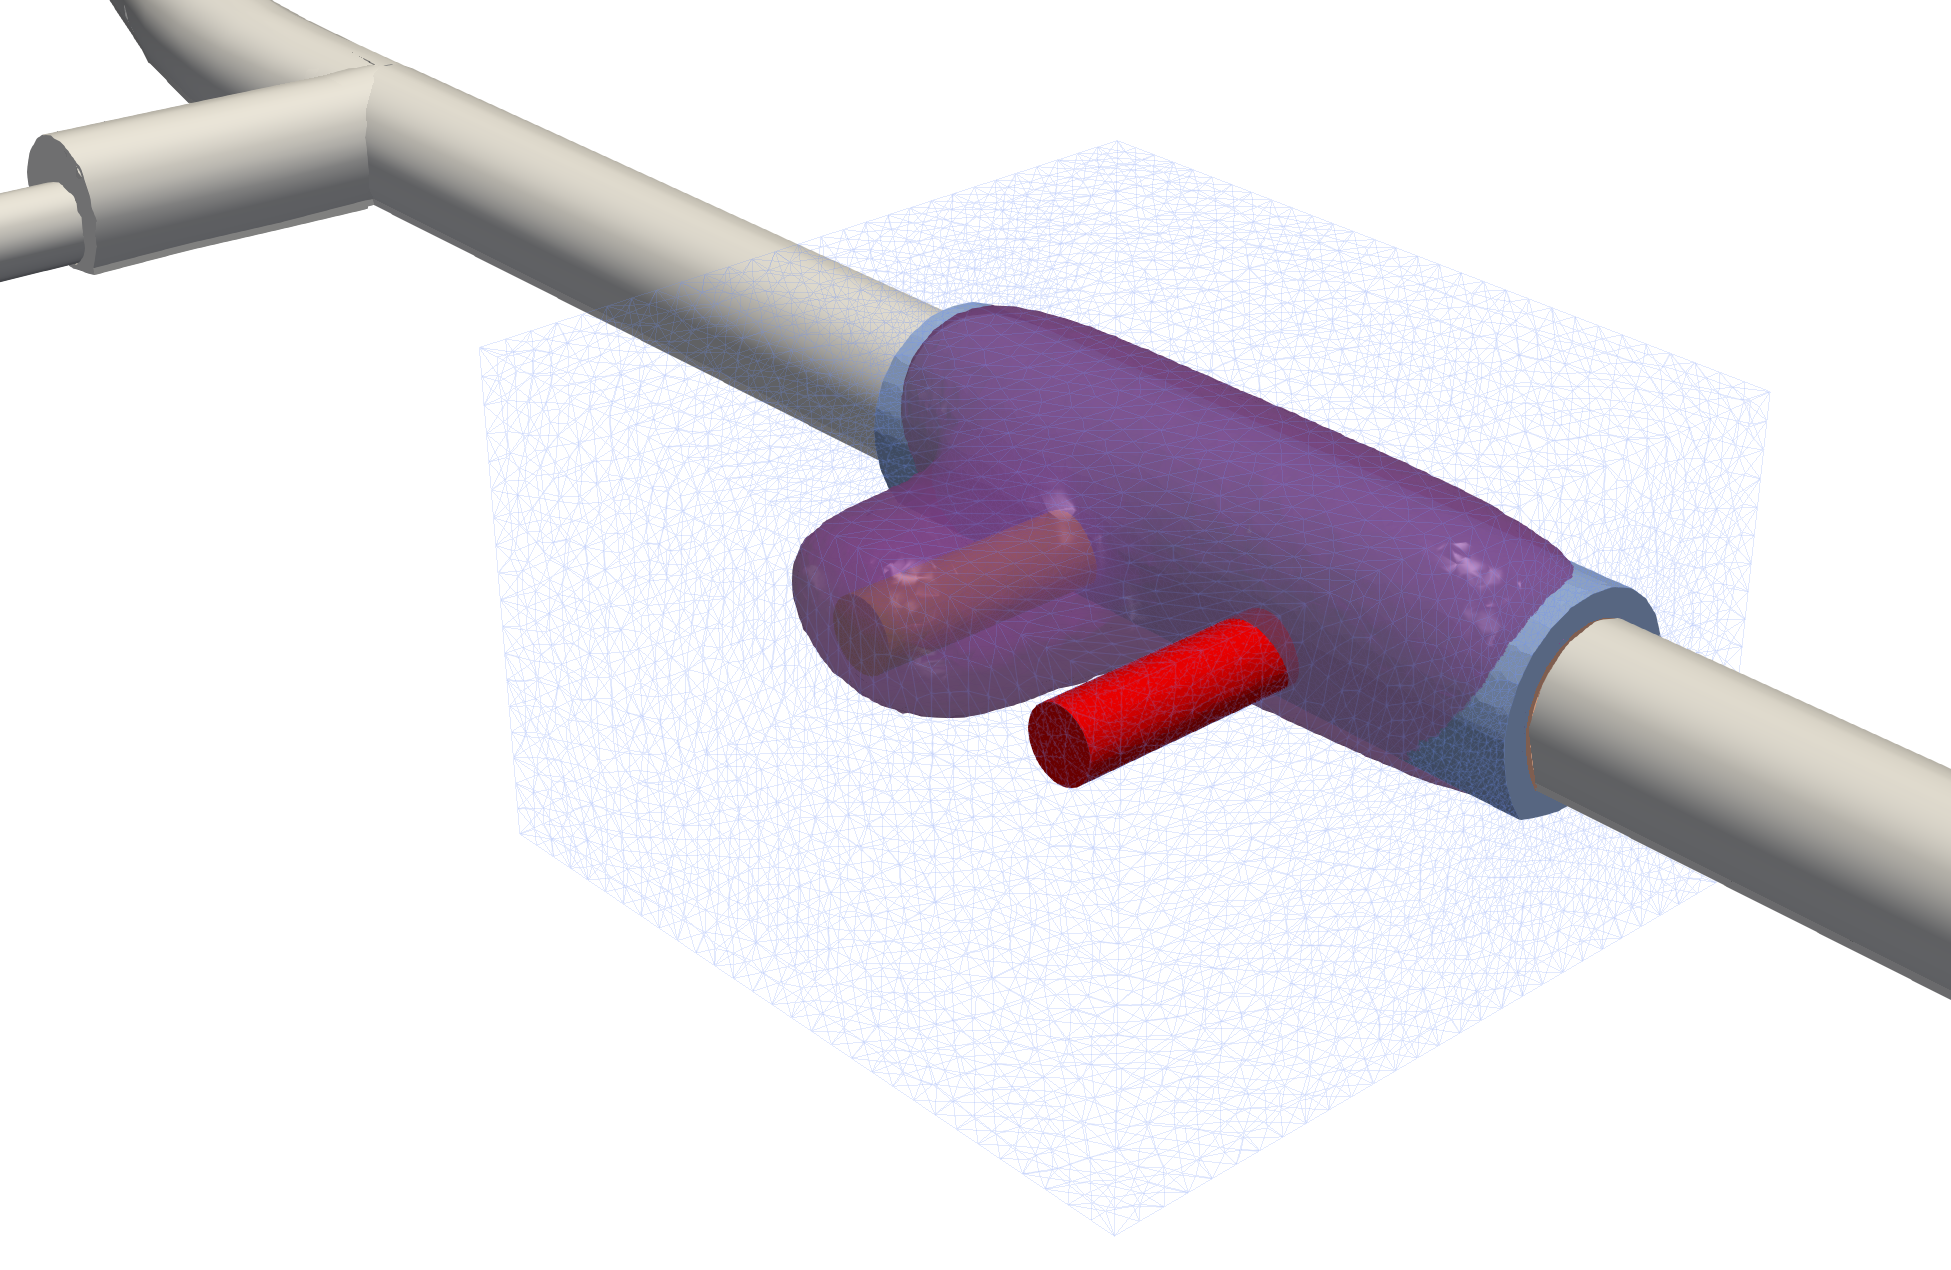
\includegraphics[width=0.49\textwidth]{figures/cd-a}
\caption{Virtualization of the CD-A experiment (Source: BGR/UFZ)}
\label{fig:cd-a}
\end{wrapfigure}
The procedure will be explained using the example of the CD-A experiment in the underground laboratory at Mt. Terri (see section \ref{sec:wp1-plan}). In the first project phase, the constitutive model was developed and implemented \cite{Vowinckel2019}. In order to use the models as realistically as possible, they are built into the underground laboratory using virtualization (see figure \ref{fig:cd-a}). The model has already been used for the planning of the CD-A experiment to determine the optimal distance between the niches (no significant interaction within 20 years). A further increase of the process complexity (nonlinear mechanics in the HM context) requires the unconditional use of HPC methods to simulate a large number of variants. The model results should be continuously compared with the running experiments and also integrated into the existing virtualization context. This is the basic idea of continuous data and model integration.


